%!TEX root = ../main.tex

\section{Design} % (fold)
\label{sec:design}

Now that the list of requirements have been created, it is time to create a plan of how the product is going to fulfill these requirements. 
When that has been done the weather categories has to be delimited into a realistic amount of weather conditions. 
After that the visual and audial elements have to be found by pre-testing. 
In the end when the sounds and pictures have been found it is time to create the blueprint of how the pictures should look like and how the sounds is going to be created.

\begin{figure}[!htbp]
    \centering
    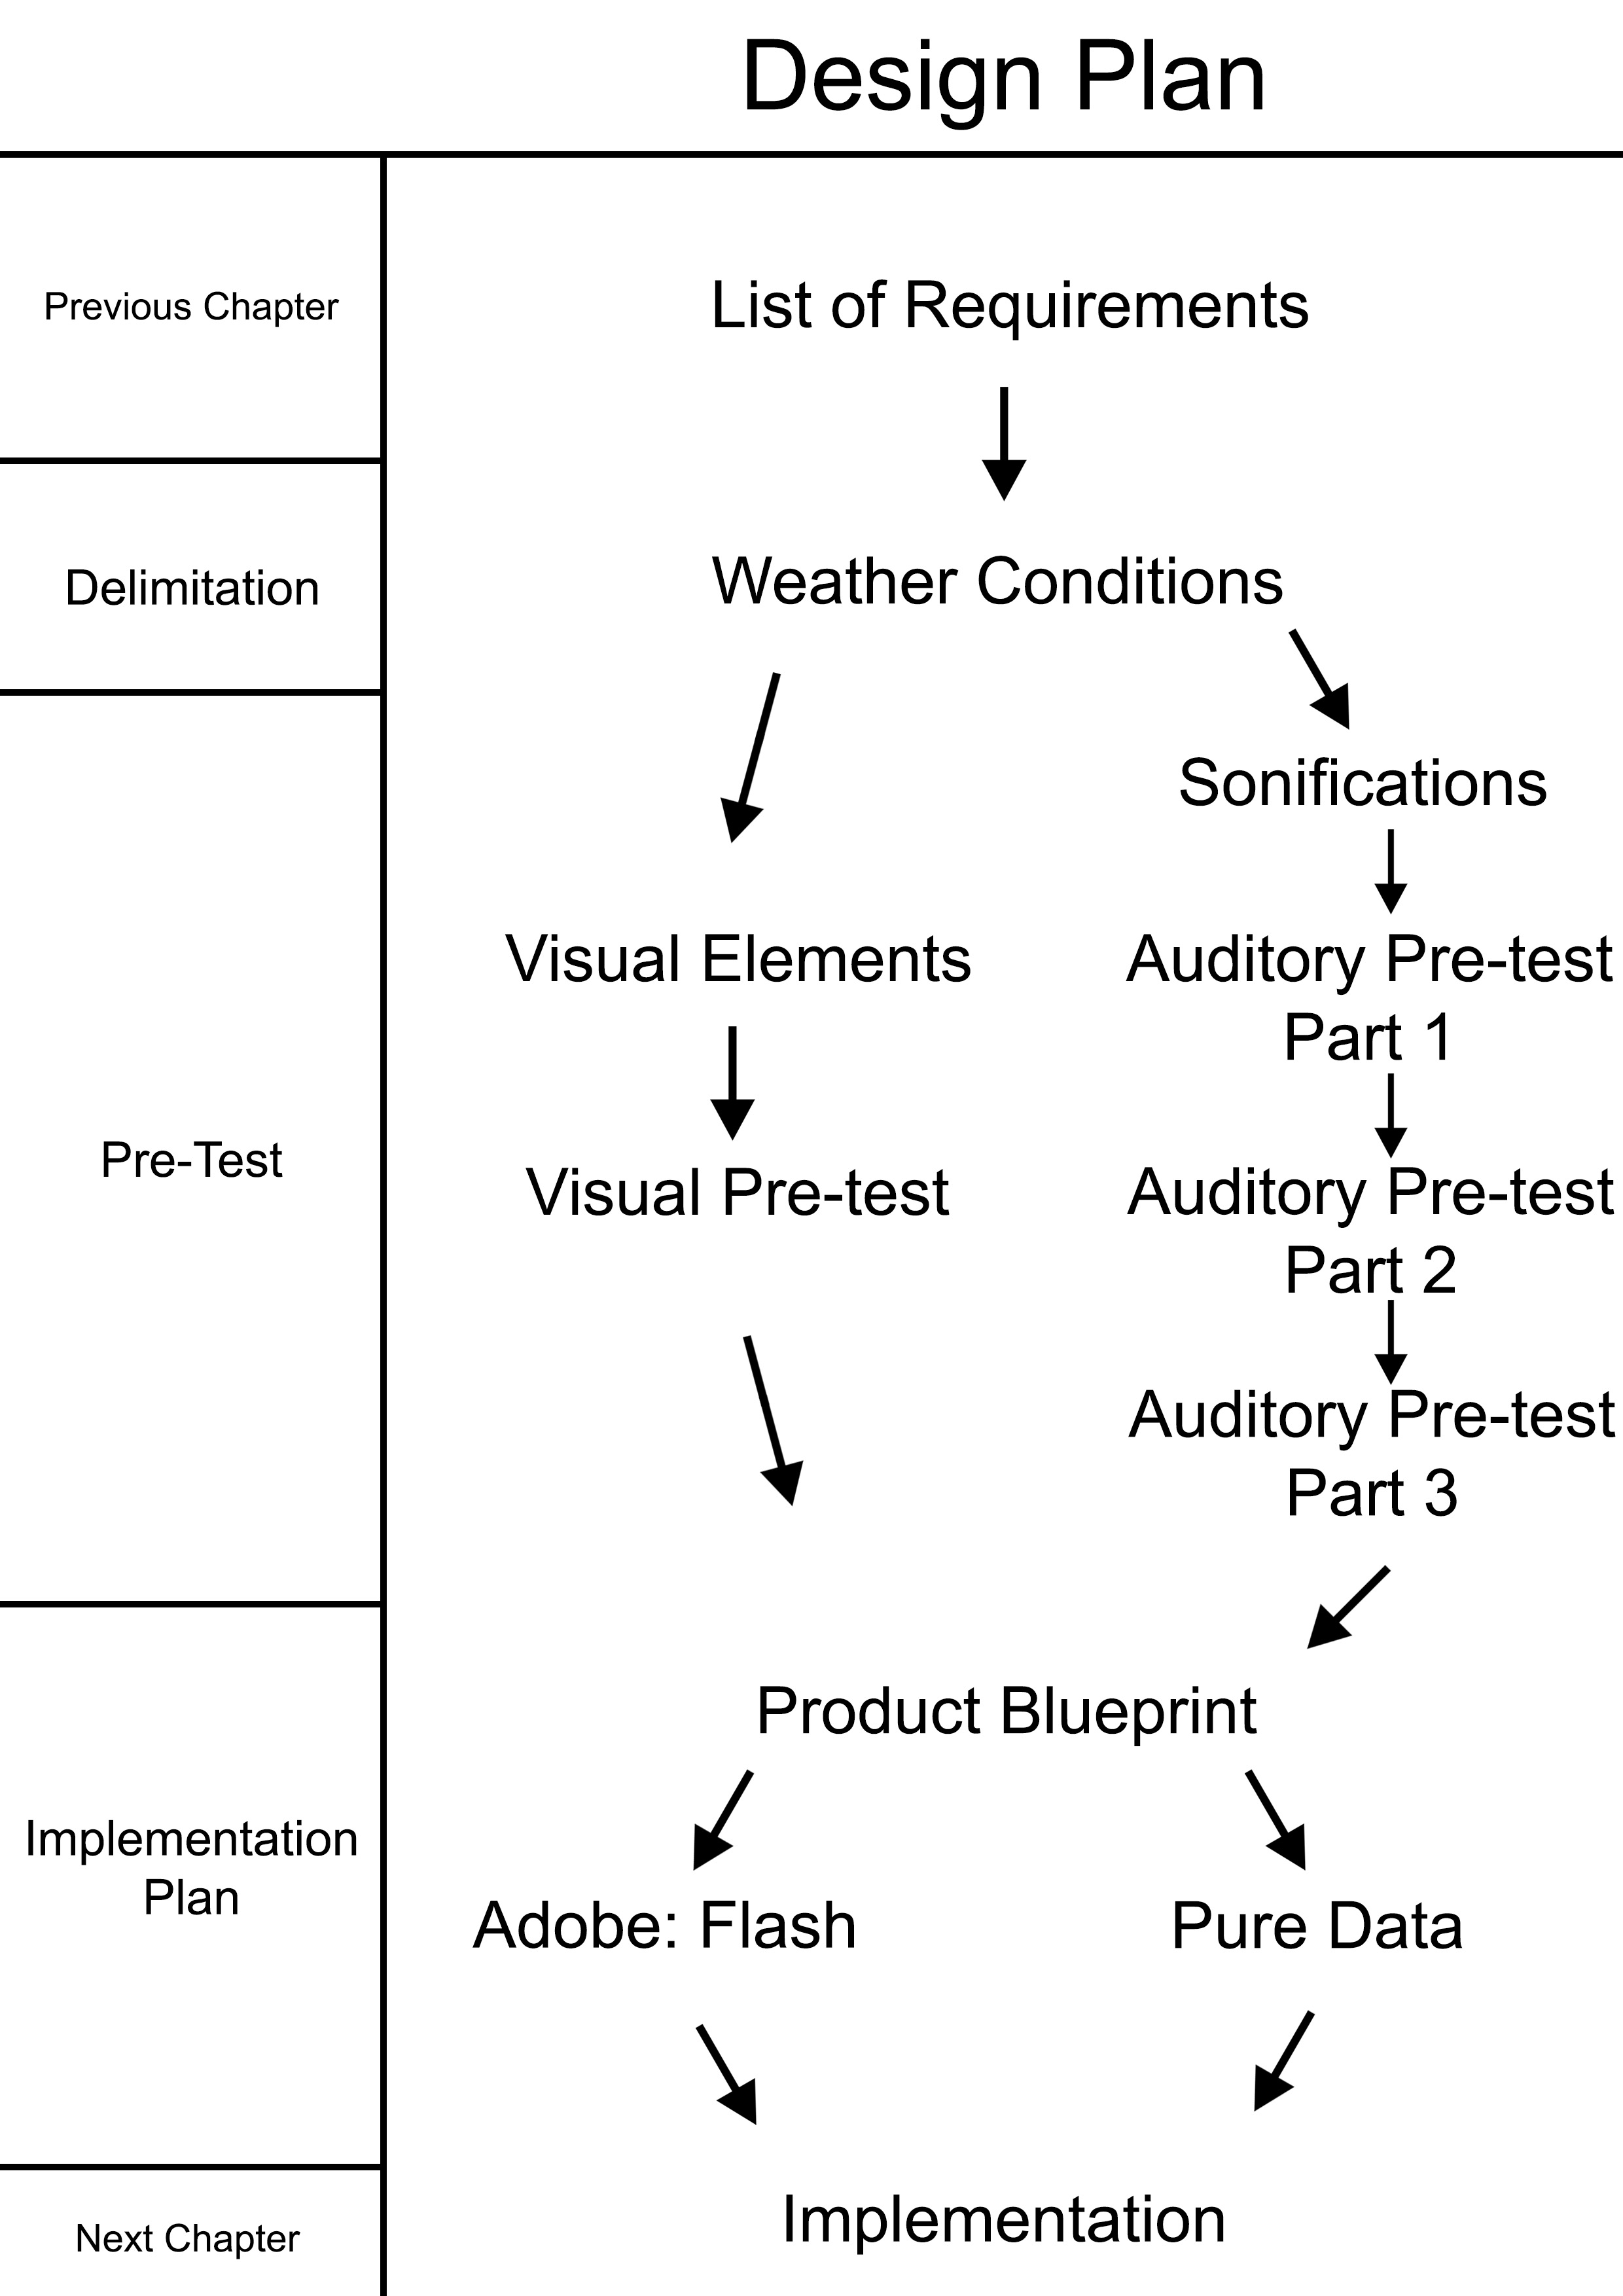
\includegraphics[width=.5\textwidth]{images/Design1.jpg}
    \caption{Plan for design process}
    \label{fig:design1}
\end{figure}


\subsection*{A design to meet all the requirements} % (fold)
\label{sub:a_design_to_meet_all_the_requirements}



% subsection a_design_to_meet_all_the_requirements (end)


\subsection*{Weather Conditions} % (fold)
\label{sub:weather_conditions}

There are a lot of different kinds of weather data. 
Since it is not possible to cover every single category of weather data within the projects time limit, we made the decision to make a delimitation of the categories.


Based on the research from the weather applications the following raw weather data list was created.

\subsubsection*{Raw list of weather data} % (fold)
\label{ssub:raw_list_of_weather_data}

\begin{itemize}
     \item \textbf{Temperature/Dewpoint} - Current air temperature 2 meters above terrain.
     \item \textbf{Wind speed} - Average wind speed over 10 minutes, 10 meters above terrain.
     \item \textbf{Wind direction} - Average wind direction in degrees.
     \item \textbf{Air pressure} - Pressure at sea level measured i hPa (Hectopascal).
     \item \textbf{Humidity} - Current relative humidity measured 2 meters above terrain, measured in percent.
     \item \textbf{Precipitation} - Rain/sleet/snow/hail over the past ten minutes measured in mm.
     \item \textbf{Sun hours} - Hours with sun in a day.
     \item \textbf{Pollen Forecast} - The potency of the pollen. 
     \item \textbf{Sunrise / sunset} - Time of day where the sun rises and sets.
     \item \textbf{Cloud cover}
     \item \textbf{Wind chill} - The winds effect on air temperature.
     \item \textbf{Visibility} - How far can you see with clear line of sight.
     \item \textbf{UV-index} - Intensity of UV radiation.
     \item \textbf{Fronts} 
     \item \textbf{Source Regions} - Where the air is coming from.
     \item \textbf{Drought} - Risk of drought. Presented as a scale.
 \end{itemize}

After going through the data on the raw list we found that many of the weather categories didn’t suit into our project. 
So we decided to only taking relevant weather data that people normally would use in an everyday situation.

% subsubsection raw_list_of_weather_data (end)


\subsubsection*{List of relevant data} % (fold)
\label{ssub:list_of_relevant_data}

\begin{itemize}
     \item \textbf{Temperature/Dewpoint} - Current air temperature 2 meters above terrain.
     \item \textbf{Wind speed} - Average wind speed over 10 minutes, 10 meters above terrain.
     \item \textbf{Wind direction} - Average wind direction in degrees.
     \item \textbf{Humidity} - Current relative humidity measured 2 meters above terrain, measured in percent.
     \item \textbf{Precipitation} - Rain/sleet/snow/hail over the past ten minutes measured in mm.
     \item \textbf{Sun hours} - Hours with sun in a day.
     \item \textbf{Pollen Forecast} - The potency of the pollen.
     \item \textbf{Wind chill} - The winds effect on air temperature.
     \item \textbf{Visibility} - How far can you see with clear line of sight.
     \item \textbf{UV-index} - Intensity of UV radiation.
 \end{itemize}

After going through the relevant weather data we decided that the list still was too long and could create problems further into problems with our time limit. 
So in order to keep the schedule and not create a long and boring test, we decided to make a delimited list. 
This list was based on what an average person would need to know in an everyday scenario.

% subsubsection list_of_relevant_data (end)


\subsubsection*{List of delimited weather data} % (fold)
\label{ssub:list_of_delimited_weather_data}

\begin{itemize}
     \item \textbf{Temperature/Dewpoint} - Current air temperature 2 meters above terrain.
     \item \textbf{Wind speed} - Average wind speed over 10 minutes, 10 meters above terrain.
     \item \textbf{Precipitation} - Rain/sleet/snow/hail over the past ten minutes measured in mm.
     \item \textbf{Pollen Forecast} - The potency of the pollen.
     \item \textbf{Visibility} - How far can you see with clear line of sight.
     \item \textbf{Cloud Cover.}
 \end{itemize}

% subsubsection list_of_delimited_weather_data (end)


\subsubsection{Categories} % (fold)
\label{ssub:categories}

Now that the list is has been delimited it has to be converted into a design that makes sure it’s easy for the people performing our test to answer on our questions. 
It’s hard for people to connect with numbers example: “Could you make a sound based on a temperature on 12 degrees” and since it’s not possible for us to go through every degree, the numbers were converted into three categories: Low, Medium and High. 
We also decided that the following weather data: Pollen and Visibility should act like a warning indicator. 
This means that the sound should only be played above or below a specific value.

% subsubsection categories (end)

% subsection weather_conditions (end)

\subsection{Visual pre-test} % (fold)
\label{sub:visual_pre_test}



% subsection visual_pre_test (end)


\subsection{Sound pre-test} % (fold)
\label{sub:sound_pre_test}

% subsection sound_pre_test (end)


\subsection{Product Blueprint} % (fold)
\label{sub:product_blueprint}

Now that the visual and audio elements have been found, it is time for us to plan how to make use of these elements.

\subsubsection{Visual Elements} % (fold)
\label{ssub:visual_elements}

Now that the visual pictures have been decided, the drawings have to be drawn and we decided to use Adobe Flash to create those pictures for the test.

% subsubsection visual_elements (end)


\subsubsection{Audio elements} % (fold)
\label{ssub:audio_elements}

Now that the different sounds for weather categories are in place, the step is to figure out how to make these sounds fit into our value categories.  
Most of the sounds can be placed and played under the fitting values but for Rain (Downpour) and Wind speed something has to be changed in order to let people know if it has a low, medium or high value. 
In order to change these sounds we have decided to use Pure Data. 
With Pure Data it is possible to change the speed of the sound and add filters so the sounds are able to fit into our value categories.  


Here is the filter we are going to use for Wind speed:


\subsubsection{Band Pass Filter} % (fold)
\label{ssub:band_pass_filter}

Band Pass Filter also called [bp~] in pure data, is a filter that allows some range of frequencies between the highest and lowest. 
It has three inputs, the first one is the input from the audio. 
The second input is for the center frequency that will be allowed to pass. 
The third input is the resonance, this determines how width the ranges of frequencies that is allowed to pass through the filter. 
The function is that the center frequency will be unchanged, but the frequencies higher or lower will be reduced or removed from the sound.

% subsubsection band_pass_filter (end)


\subsubsection{Sample} % (fold)
\label{ssub:sample}

A sample refers to a value or multiple values that is set to a point in time.

% subsubsection sample (end)


\subsubsection{Metro} % (fold)
\label{ssub:metro}

An object that keeps calling after a specific amount of time in milliseconds.

% subsubsection metro (end)
    

\subsubsection{Phasor} % (fold)
\label{ssub:phasor}

A phasor is a representation of a sinusoidal function. 
This function is based on three factors, A that is the functions amplitude, is the frequency and  is the phase.  

\begin{equation}
    A * \cos(\omega t + \theta)
\end{equation}

We use the phasor by leaving out the frequency and will only carry on the amplitude and phase. 
This leaves us with the option to add the frequency factor that through the array.

% subsubsection phasor (end)


\subsubsection{How the sound will be implemented in Pure Data} % (fold)
\label{ssub:how_the_sound_will_be_implemented_in_pure_data}

The way the sound will be implemented in pure data and will go through a six or seven step process.

\begin{enumerate}
    \item Input Sound
    \item Array / Sample
    \item Determine Sample Speed
    \item Phasor
    \item Merge Array and Sample Speed
    \item Fliter
    \item Output Sound
\end{enumerate}

First step is to make sure that the sound will be imported into the program. 
Second step is to send the sound into an array that will split the sound into samples. 
The third step is to detect how fast the samples normally are going to be played in order to create the same sound. 
The fourth step is sending the sample speed into a Phasor. 
The fifth step is to merge the the play speed from the phasor with the array with the samples. 
This will create the sound based on the play speed that has been changed. 
The sixth step is only to be implemented if a filter is required for the sound. 
The seventh and last step is the output sound that have been going through all the new changes and will now sound differently.

% subsubsection how_the_sound_will_be_implemented_in_pure_data (end)

% subsubsection audio_elements (end)

% subsection product_blueprint (end)

% section design (end)